\resizebox{\columnwidth}{!}{%
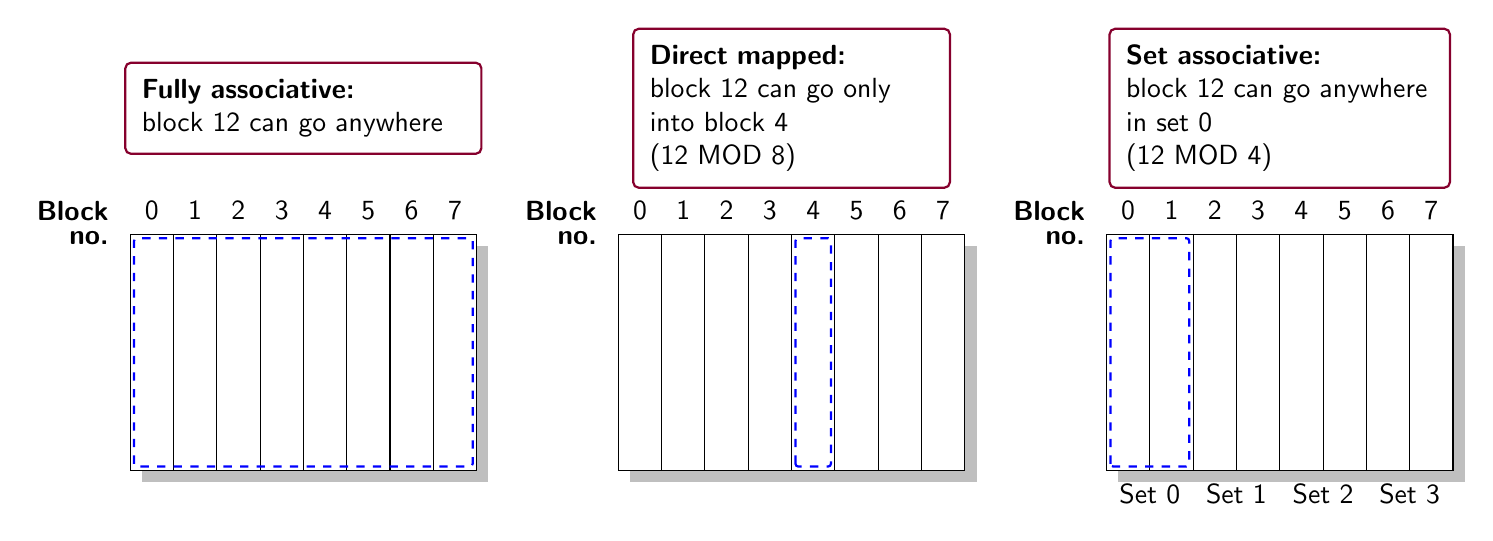
\begin{tikzpicture}[
    every node/.style={font=\sffamily},
    titlebox/.style={
        draw=purple!70!black,
        thick,
        rounded corners=2pt,
        fill=white,
        align=left,
        inner sep=6pt,
        text width=4.1cm
    }
]

% ---------- macro to draw one cache diagram ----------
% #1 = x offset
% #2 = highlight drawing commands
% #3 = extra labels (e.g. set labels)
\newcommand{\cachediagram}[3]{
  \begin{scope}[xshift=#1]
    % shadow rectangle (offset behind)
    \fill[gray!50] (0.15,-0.15) rectangle (4.55,2.85);
    % main cache rectangle
    \fill[white] (0,0) rectangle (4.4,3.0);
    \draw[black] (0,0) rectangle (4.4,3.0);
    % 8 vertical dividers -> 8 blocks
    \foreach \i in {1,...,7}{
        \draw[black] (\i*0.55,0) -- (\i*0.55,3.0);
    }
    % block numbers on top
    \foreach \i in {0,...,7}{
        \node at (\i*0.55+0.275, 3.3) {\i};
    }
    % highlight
    #2
    % labels
    \node[anchor=east] at (-0.15,3.3) {\textbf{Block}};
    \node[anchor=east] at (-0.15,2.95) {\textbf{no.}};
    % \node[anchor=east] at (-0.15,-0.6) {\textbf{Cache}};
    #3
  \end{scope}
}

% ---------- Diagram 1: Fully associative (all 8 blocks highlighted) ----------
\cachediagram{0cm}{
    \draw[blue, dashed, thick, rounded corners=1pt] (0.05,0.05) rectangle (4.35,2.95);
}{}

\node[titlebox] at (2.2,4.6) {\textbf{Fully associative:}\\ block 12 can go anywhere};

% ---------- Diagram 2: Direct mapped (block 4 only) ----------
\cachediagram{6.2cm}{
    \draw[blue, dashed, thick, rounded corners=1pt] (4*0.55+0.05,0.05) rectangle (5*0.55-0.05,2.95);
}{}

\node[titlebox, text width=3.6cm] at (8.4,4.6) {\textbf{Direct mapped:}\\ block 12 can go only into block 4\\ (12 MOD 8)};

% ---------- Diagram 3: Set associative (set 0 = blocks 0,1) ----------
\cachediagram{12.4cm}{
    \draw[blue, dashed, thick, rounded corners=1pt] (0.05,0.05) rectangle (2*0.55-0.05,2.95);
}{
    \node at (0.55,-0.3) {Set 0};
    \node at (1.65,-0.3) {Set 1};
    \node at (2.75,-0.3) {Set 2};
    \node at (3.85,-0.3) {Set 3};
}

\node[titlebox, text width=3.9cm] at (14.6,4.6) {\textbf{Set associative:}\\ block 12 can go anywhere in set 0\\ (12 MOD 4)};

\end{tikzpicture}
}